
\documentclass[11pt]{book}
\usepackage{graphicx}
\begin{document}

\section{
Geometron Presents Geometron}

\begin{figure}

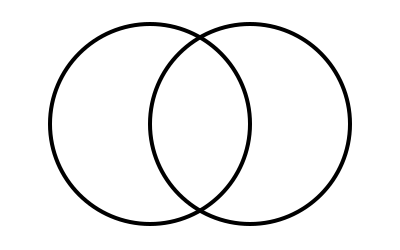
\includegraphics[width=\linewidth]{../figures/vesica.png}

\caption{Vesica Pisces.  The "hello, world" of geometric languages}
\end{figure}


\begin{figure}

\includegraphics[width=\linewidth]{../figures/vesicacode.png}

\caption{Symbols which spell out the vesica pisces. Each symbol represents a geometric action, and they are: draw circle of radius "side", move right by "side", draw circle of radius "side".}
\end{figure}


\begin{figure}

\includegraphics[width=\linewidth]{../figures/squarecircles.png}

\caption{If we can move and draw circles, we can draw more, on the default square lattice.}
\end{figure}


\begin{figure}

\includegraphics[width=\linewidth]{../figures/squarecirclescode.png}

\caption{Code to construct the four circles}
\end{figure}


\begin{figure}

\includegraphics[width=\linewidth]{../figures/triangle1.png}

\caption{Equilateral triangle, which uses 6 fold symmetry to get a 60 degree angle, after using the 90 degree symmetry to rotate so it has a horizontal bottom side.}
\end{figure}


\begin{figure}

\includegraphics[width=\linewidth]{../figures/spelltriangle1.png}

\caption{This shows how we make closed paths using Geometron: there are several ways to terminate a path, including a filled path, a closed unfilled path which is shown, and a open unfilled path.  These seems like small differences but will make a large impact on how our symbols look.}
\end{figure}


\begin{figure}

\includegraphics[width=\linewidth]{../figures/trianglefractal1.png}

\caption{Sequence of triangle each 2x smaller than prvious one.}
\end{figure}


\begin{figure}

\includegraphics[width=\linewidth]{../figures/triangle1fractalspell.png}

\caption{Symbol glyph spelling for triangular fractal.}
\end{figure}


\begin{figure}

\includegraphics[width=\linewidth]{../figures/spelltriangleshape.png}

\caption{Spelling of triangle shape used for fractal.}
\end{figure}


\begin{figure}

\includegraphics[width=\linewidth]{../figures/koch0.png}

\caption{This symbol breaks a segment into three parts and makes a triangle out from the middle part. it is a fundamental element of the Koch Curve, which we shall now construct.}
\end{figure}


\begin{figure}

\includegraphics[width=\linewidth]{../figures/koch1.png}

\caption{Spelling of the above symbol, along with its symbol glyph.}
\end{figure}


\begin{figure}

\includegraphics[width=\linewidth]{../figures/koch2.png}

\caption{Spelling of the next iteration.  Each iteration is the same size as the previous one but the number of segments goes up exponentially, so we only need to do this a few times.}
\end{figure}


\begin{figure}

\includegraphics[width=\linewidth]{../figures/koch3.png}

\caption{And finally a Koch Curve, with enough levels of zoom that the non-fractal nature is lost in pixel size in the screen.  This highlights a very annoying aspect of Mandelbrot's book: the work there exists in a fantasy world where infinite scales exist in both large and small directions, unbounded by physical pixels, numerical registers, atoms etc.  Geomtron always ties as closely as possible to physical pixels on a screen, dispensing with such fantasies.}
\end{figure}


\begin{figure}

\includegraphics[width=\linewidth]{../figures/root2triangle1.png}

\caption{Fractal triangle illustrating square root of two scaling and bisection action which goes from 90 degrees to 45 degrees. }
\end{figure}


\begin{figure}

\includegraphics[width=\linewidth]{../figures/spelltriangle45.png}

\caption{Spelling of 45 degree fractal.  This could be made shorter by using a 135 degree angle, but I chose simplicity over brevity and each 135 degree turn is expressed as three 45 degree turns.}
\end{figure}



\begin{figure}

\includegraphics[width=\linewidth]{../figures/golden1.png}

\caption{The Golden Triangle, an isosceles triangle with 36 degrees ,72 and 72 degrees, with sides equal to the base times $\phi = \frac{\sqrt{5}+1}{2}$}
\end{figure}


\begin{figure}

\includegraphics[width=\linewidth]{../figures/spellgolden1.png}

\caption{Spelling of Golden Triangle showing the symbol glyphs to denote Golden Ratio for scaling and five fold symmetry to get 72 degrees, then a bisect action which gets from 72 to 36 degrees.}
\end{figure}



\end{document}
